\documentclass{article}
\usepackage{graphicx} % Required for inserting images
\usepackage{listings}

\title{HPC-Master.Lab3}
\author{Phan Thanh Bình}
\date{September 2026}

\setlength{\parindent}{0pt}
\setlength{\parskip}{3pt}

\begin{document}

\maketitle

\section{Labwork Implementation}
Here is the image that I chose for this labwork, with the size of 900 x 550.
\begin{figure}[h]
    \centering
    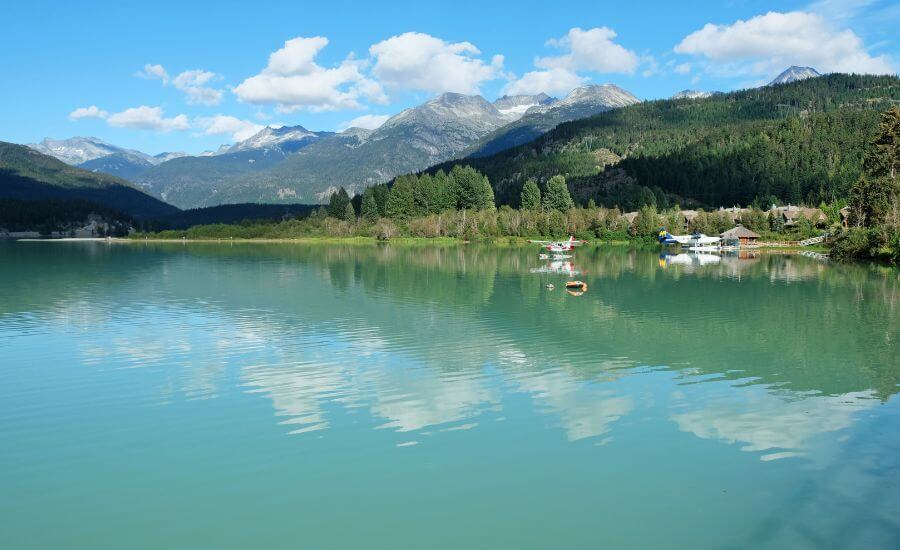
\includegraphics[width=0.5\linewidth]{green-lake-small.jpg}
    \caption{Source Image}
    \label{fig:src}
\end{figure}

And below is the code I made. The GPU-version I copied directly from the slides. The CPU-version is basically identical, with a minor difference that instead of taking the average of RGB values (sum and divide), I multiply the RGB values with its weight (in this case $1/3$ each) then take the sum. This is due to numpy \textit{uint8} overflow mechanism, but GPU-version does not suffer from this problem - probably due to the cuda.jit has already done some optimizations.

\begin{verbatim}
def cpu_grayscale(src, dst):
  for x in range(src.shape[0]):
    g = np.uint8(src[x, 0] * R + src[x, 1] * B + src[x, 2] * G)
    dst[x, 0] = dst[x, 1] = dst[x, 2] = g

@cuda.jit
def gpu_grayscale(src, dst):
  tidx = cuda.threadIdx.x + cuda.blockIdx.x * cuda.blockDim.x
  g = np.uint8((src[tidx, 0] + src[tidx, 1] + src[tidx, 2]) / 3)
  dst[tidx, 0] = dst[tidx, 1] = dst[tidx, 2] = g
\end{verbatim}

To summarize the flow: For each \textbf{source} pixel position, compute the average of the values from 3 channels RGB, then copy the result to the 3 channels of the \textbf{destination} at the same pixel position.

\paragraph{Speedup Measurement}
To measure the time carried out by CPU and GPU version, need 2 markers: $start\_time$ and $end\_time$ the take the subtraction. The decision here is where to place those 2 markers, or which codes is included in the measurement. For that, I did as follows, the idea is that both start with source image on host and finish with the destination image on host.
\begin{itemize}
\item CPU: allocate $dst$ on host, convert function
\item GPU: allocate $dst$ on device, copy $src$ from host to device, convert function, copy $dst$ from device to host
\end{itemize}

And the result show a considerable speedup when running the conversion on GPU. Each version is ran 5 times then takes the average.
\begin{itemize}
\item CPU $\approx 3.7s$
\item GPU $\approx 0.07s$
\end{itemize}

\section{Block Size Experiment}
Since the previous used image too small for GPU which makes it hard to observe the differences between block sizes, I have decided to use a bigger image for this experiment. I achieved this simply via $cv2.resize$, with each height and width got upscale by 10 times.

The blocks sizes that I chose are powers of two. i.e $(8, 16, 32, ...)$. Each run with a block size is repeated 20 times, and the average execution time is used for comparison. Additionally, after each run I use the \textbf{del}keyword in Python with the expect to free the memory allocated for each run.

Below is the comparison graph that I drawn. The trend is quite clear as there is a significant improvement from 8 to 64, but increasing beyond 64 shows no benefits. So my conclusion is there must be some sort of \textit{'optimal'} value for the block size, too small cause the performance drop and too big might cause some other tradeoffs.
\begin{figure}[h]
    \centering
    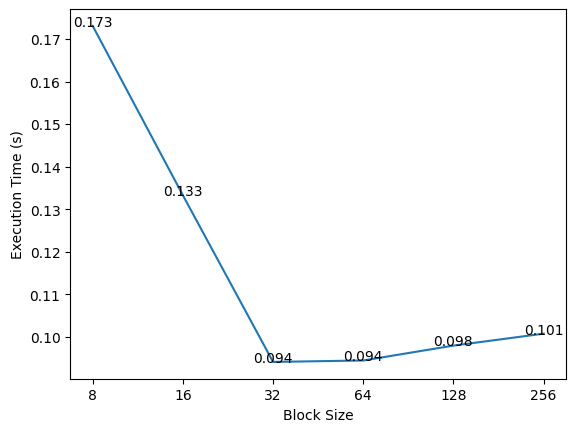
\includegraphics[width=\linewidth]{compare-graph.png}
    \caption{Block Size Benchmark Graph}
    \label{fig:compare-graph}
\end{figure}

\end{document}
